\documentclass[1p]{elsarticle_modified}
%\bibliographystyle{elsarticle-num}

%\usepackage[colorlinks]{hyperref}
%\usepackage{abbrmath_seonhwa} %\Abb, \Ascr, \Acal ,\Abf, \Afrak
\usepackage{amsfonts}
\usepackage{amssymb}
\usepackage{amsmath}
\usepackage{amsthm}
\usepackage{scalefnt}
\usepackage{amsbsy}
\usepackage{kotex}
\usepackage{caption}
\usepackage{subfig}
\usepackage{color}
\usepackage{graphicx}
\usepackage{xcolor} %% white, black, red, green, blue, cyan, magenta, yellow
\usepackage{float}
\usepackage{setspace}
\usepackage{hyperref}

\usepackage{tikz}
\usetikzlibrary{arrows}

\usepackage{multirow}
\usepackage{array} % fixed length table
\usepackage{hhline}

%%%%%%%%%%%%%%%%%%%%%
\makeatletter
\renewcommand*\env@matrix[1][\arraystretch]{%
	\edef\arraystretch{#1}%
	\hskip -\arraycolsep
	\let\@ifnextchar\new@ifnextchar
	\array{*\c@MaxMatrixCols c}}
\makeatother %https://tex.stackexchange.com/questions/14071/how-can-i-increase-the-line-spacing-in-a-matrix
%%%%%%%%%%%%%%%

\usepackage[normalem]{ulem}

\newcommand{\msout}[1]{\ifmmode\text{\sout{\ensuremath{#1}}}\else\sout{#1}\fi}
%SOURCE: \msout is \stkout macro in https://tex.stackexchange.com/questions/20609/strikeout-in-math-mode

\newcommand{\cancel}[1]{
	\ifmmode
	{\color{red}\msout{#1}}
	\else
	{\color{red}\sout{#1}}
	\fi
}

\newcommand{\add}[1]{
	{\color{blue}\uwave{#1}}
}

\newcommand{\replace}[2]{
	\ifmmode
	{\color{red}\msout{#1}}{\color{blue}\uwave{#2}}
	\else
	{\color{red}\sout{#1}}{\color{blue}\uwave{#2}}
	\fi
}

\newcommand{\Sol}{\mathcal{S}} %segment
\newcommand{\D}{D} %diagram
\newcommand{\A}{\mathcal{A}} %arc


%%%%%%%%%%%%%%%%%%%%%%%%%%%%%5 test

\def\sl{\operatorname{\textup{SL}}(2,\Cbb)}
\def\psl{\operatorname{\textup{PSL}}(2,\Cbb)}
\def\quan{\mkern 1mu \triangleright \mkern 1mu}

\theoremstyle{definition}
\newtheorem{thm}{Theorem}[section]
\newtheorem{prop}[thm]{Proposition}
\newtheorem{lem}[thm]{Lemma}
\newtheorem{ques}[thm]{Question}
\newtheorem{cor}[thm]{Corollary}
\newtheorem{defn}[thm]{Definition}
\newtheorem{exam}[thm]{Example}
\newtheorem{rmk}[thm]{Remark}
\newtheorem{alg}[thm]{Algorithm}

\newcommand{\I}{\sqrt{-1}}
\begin{document}

%\begin{frontmatter}
%
%\title{Boundary parabolic representations of knots up to 8 crossings}
%
%%% Group authors per affiliation:
%\author{Yunhi Cho} 
%\address{Department of Mathematics, University of Seoul, Seoul, Korea}
%\ead{yhcho@uos.ac.kr}
%
%
%\author{Seonhwa Kim} %\fnref{s_kim}}
%\address{Center for Geometry and Physics, Institute for Basic Science, Pohang, 37673, Korea}
%\ead{ryeona17@ibs.re.kr}
%
%\author{Hyuk Kim}
%\address{Department of Mathematical Sciences, Seoul National University, Seoul 08826, Korea}
%\ead{hyukkim@snu.ac.kr}
%
%\author{Seokbeom Yoon}
%\address{Department of Mathematical Sciences, Seoul National University, Seoul, 08826,  Korea}
%\ead{sbyoon15@snu.ac.kr}
%
%\begin{abstract}
%We find all boundary parabolic representation of knots up to 8 crossings.
%
%\end{abstract}
%\begin{keyword}
%    \MSC[2010] 57M25 
%\end{keyword}
%
%\end{frontmatter}

%\linenumbers
%\tableofcontents
%
\newcommand\colored[1]{\textcolor{white}{\rule[-0.35ex]{0.8em}{1.4ex}}\kern-0.8em\color{red} #1}%
%\newcommand\colored[1]{\textcolor{white}{ #1}\kern-2.17ex	\textcolor{white}{ #1}\kern-1.81ex	\textcolor{white}{ #1}\kern-2.15ex\color{red}#1	}

{\Large $\underline{12a_{1089}~(K12a_{1089})}$}

\setlength{\tabcolsep}{10pt}
\renewcommand{\arraystretch}{1.6}
\vspace{1cm}\begin{tabular}{m{100pt}>{\centering\arraybackslash}m{274pt}}
\multirow{5}{120pt}{
	\centering
	\includegraphics[width=112pt]{../../../GIT/diagram.site/Diagrams/png/1890_12a_1089.png}\\
\ \ \ A knot diagram\footnotemark}&
\allowdisplaybreaks
\textbf{Linearized knot diagam} \\
\cline{2-2}
 &
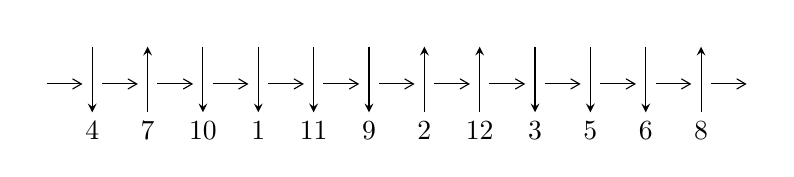
\begin{tikzpicture}[x=20pt, y=17pt]
	% nodes
	\node (C0) at (0, 0) {};
	\node (C1) at (1, 0) {};
	\node (C1U) at (1, +1) {};
	\node (C1D) at (1, -1) {4};

	\node (C2) at (2, 0) {};
	\node (C2U) at (2, +1) {};
	\node (C2D) at (2, -1) {7};

	\node (C3) at (3, 0) {};
	\node (C3U) at (3, +1) {};
	\node (C3D) at (3, -1) {10};

	\node (C4) at (4, 0) {};
	\node (C4U) at (4, +1) {};
	\node (C4D) at (4, -1) {1};

	\node (C5) at (5, 0) {};
	\node (C5U) at (5, +1) {};
	\node (C5D) at (5, -1) {11};

	\node (C6) at (6, 0) {};
	\node (C6U) at (6, +1) {};
	\node (C6D) at (6, -1) {9};

	\node (C7) at (7, 0) {};
	\node (C7U) at (7, +1) {};
	\node (C7D) at (7, -1) {2};

	\node (C8) at (8, 0) {};
	\node (C8U) at (8, +1) {};
	\node (C8D) at (8, -1) {12};

	\node (C9) at (9, 0) {};
	\node (C9U) at (9, +1) {};
	\node (C9D) at (9, -1) {3};

	\node (C10) at (10, 0) {};
	\node (C10U) at (10, +1) {};
	\node (C10D) at (10, -1) {5};

	\node (C11) at (11, 0) {};
	\node (C11U) at (11, +1) {};
	\node (C11D) at (11, -1) {6};

	\node (C12) at (12, 0) {};
	\node (C12U) at (12, +1) {};
	\node (C12D) at (12, -1) {8};
	\node (C13) at (13, 0) {};

	% arrows
	\draw[->,>={angle 60}]
	(C0) edge (C1) (C1) edge (C2) (C2) edge (C3) (C3) edge (C4) (C4) edge (C5) (C5) edge (C6) (C6) edge (C7) (C7) edge (C8) (C8) edge (C9) (C9) edge (C10) (C10) edge (C11) (C11) edge (C12) (C12) edge (C13) ;	\draw[->,>=stealth]
	(C1U) edge (C1D) (C2D) edge (C2U) (C3U) edge (C3D) (C4U) edge (C4D) (C5U) edge (C5D) (C6U) edge (C6D) (C7D) edge (C7U) (C8D) edge (C8U) (C9U) edge (C9D) (C10U) edge (C10D) (C11U) edge (C11D) (C12D) edge (C12U) ;
	\end{tikzpicture} \\
\hhline{~~} \\& 
\textbf{Solving Sequence} \\ \cline{2-2} 
 &
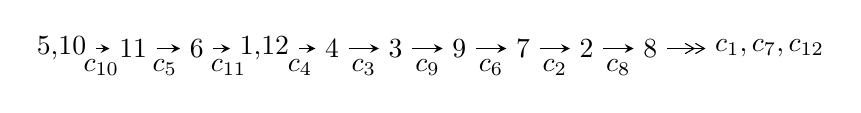
\begin{tikzpicture}[x=23pt, y=7pt]
	% node
	\node (A0) at (-1/8, 0) {5,10};
	\node (A1) at (1, 0) {11};
	\node (A2) at (2, 0) {6};
	\node (A3) at (49/16, 0) {1,12};
	\node (A4) at (33/8, 0) {4};
	\node (A5) at (41/8, 0) {3};
	\node (A6) at (49/8, 0) {9};
	\node (A7) at (57/8, 0) {7};
	\node (A8) at (65/8, 0) {2};
	\node (A9) at (73/8, 0) {8};
	\node (C1) at (1/2, -1) {$c_{10}$};
	\node (C2) at (3/2, -1) {$c_{5}$};
	\node (C3) at (5/2, -1) {$c_{11}$};
	\node (C4) at (29/8, -1) {$c_{4}$};
	\node (C5) at (37/8, -1) {$c_{3}$};
	\node (C6) at (45/8, -1) {$c_{9}$};
	\node (C7) at (53/8, -1) {$c_{6}$};
	\node (C8) at (61/8, -1) {$c_{2}$};
	\node (C9) at (69/8, -1) {$c_{8}$};
	\node (A10) at (11, 0) {$c_{1},c_{7},c_{12}$};

	% edge
	\draw[->,>=stealth]	
	(A0) edge (A1) (A1) edge (A2) (A2) edge (A3) (A3) edge (A4) (A4) edge (A5) (A5) edge (A6) (A6) edge (A7) (A7) edge (A8) (A8) edge (A9) ;
	\draw[->>,>={angle 60}]	
	(A9) edge (A10);
\end{tikzpicture} \\ 

\end{tabular} \\

\footnotetext{
The image of knot diagram is generated by the software ``\textbf{Draw programme}" developed by Andrew Bartholomew(\url{http://www.layer8.co.uk/maths/draw/index.htm\#Running-draw}), where we modified some parts for our purpose(\url{https://github.com/CATsTAILs/LinksPainter}).
}\phantom \\ \newline 
\centering \textbf{Ideals for irreducible components\footnotemark of $X_{\text{par}}$} 
 
\begin{align*}
I^u_{1}&=\langle 
2.16790\times10^{353} u^{115}+2.84497\times10^{353} u^{114}+\cdots+2.63757\times10^{354} b+1.97507\times10^{355},\\
\phantom{I^u_{1}}&\phantom{= \langle  }-3.27005\times10^{354} u^{115}-5.00102\times10^{354} u^{114}+\cdots+1.23966\times10^{356} a-4.07845\times10^{356},\\
\phantom{I^u_{1}}&\phantom{= \langle  }u^{116}+u^{115}+\cdots+77 u-47\rangle \\
I^u_{2}&=\langle 
-527881694 u^{37}+532329791 u^{36}+\cdots+163338409 b-249206027,\\
\phantom{I^u_{2}}&\phantom{= \langle  }-867853410 u^{37}+1532845572 u^{36}+\cdots+163338409 a-1189450516,\;u^{38}-22 u^{36}+\cdots+2 u+1\rangle \\
\\
\end{align*}
\raggedright * 2 irreducible components of $\dim_{\mathbb{C}}=0$, with total 154 representations.\\
\footnotetext{All coefficients of polynomials are rational numbers. But the coefficients are sometimes approximated in decimal forms when there is not enough margin.}
\newpage
\renewcommand{\arraystretch}{1}
\centering \section*{I. $I^u_{1}= \langle 2.17\times10^{353} u^{115}+2.84\times10^{353} u^{114}+\cdots+2.64\times10^{354} b+1.98\times10^{355},\;-3.27\times10^{354} u^{115}-5.00\times10^{354} u^{114}+\cdots+1.24\times10^{356} a-4.08\times10^{356},\;u^{116}+u^{115}+\cdots+77 u-47 \rangle$}
\flushleft \textbf{(i) Arc colorings}\\
\begin{tabular}{m{7pt} m{180pt} m{7pt} m{180pt} }
\flushright $a_{5}=$&$\begin{pmatrix}0\\u\end{pmatrix}$ \\
\flushright $a_{10}=$&$\begin{pmatrix}1\\0\end{pmatrix}$ \\
\flushright $a_{11}=$&$\begin{pmatrix}1\\u^2\end{pmatrix}$ \\
\flushright $a_{6}=$&$\begin{pmatrix}- u\\- u^3+u\end{pmatrix}$ \\
\flushright $a_{1}=$&$\begin{pmatrix}0.0263787 u^{115}+0.0403419 u^{114}+\cdots-3.61240 u+3.28999\\-0.0821930 u^{115}-0.107863 u^{114}+\cdots+0.687418 u-7.48822\end{pmatrix}$ \\
\flushright $a_{12}=$&$\begin{pmatrix}- u^2+1\\- u^4+2 u^2\end{pmatrix}$ \\
\flushright $a_{4}=$&$\begin{pmatrix}0.00829665 u^{115}+0.00828424 u^{114}+\cdots+14.0526 u+5.31889\\0.00131243 u^{115}+0.0121793 u^{114}+\cdots-8.59129 u-2.26904\end{pmatrix}$ \\
\flushright $a_{3}=$&$\begin{pmatrix}0.00960909 u^{115}+0.0204635 u^{114}+\cdots+5.46135 u+3.04985\\0.00131243 u^{115}+0.0121793 u^{114}+\cdots-8.59129 u-2.26904\end{pmatrix}$ \\
\flushright $a_{9}=$&$\begin{pmatrix}0.0106014 u^{115}+0.0172463 u^{114}+\cdots-16.7708 u-1.82678\\0.0306743 u^{115}+0.0473761 u^{114}+\cdots-6.13314 u+0.511842\end{pmatrix}$ \\
\flushright $a_{7}=$&$\begin{pmatrix}-0.0106968 u^{115}-0.00589435 u^{114}+\cdots+4.55965 u-2.79866\\-0.0394291 u^{115}-0.0526976 u^{114}+\cdots-4.77318 u-6.48703\end{pmatrix}$ \\
\flushright $a_{2}=$&$\begin{pmatrix}-0.0297377 u^{115}-0.0329784 u^{114}+\cdots+2.05844 u-1.66172\\-0.0542512 u^{115}-0.0727667 u^{114}+\cdots+1.99382 u-4.73724\end{pmatrix}$ \\
\flushright $a_{8}=$&$\begin{pmatrix}0.00550118 u^{115}+0.00583765 u^{114}+\cdots-11.4685 u-0.314190\\0.0190890 u^{115}+0.0342645 u^{114}+\cdots-5.58633 u-0.267695\end{pmatrix}$\\&\end{tabular}
\flushleft \textbf{(ii) Obstruction class $= -1$}\\~\\
\flushleft \textbf{(iii) Cusp Shapes $= 0.239239 u^{115}+0.274769 u^{114}+\cdots+24.2940 u+29.3306$}\\~\\
\newpage\renewcommand{\arraystretch}{1}
\flushleft \textbf{(iv) u-Polynomials at the component}\newline \\
\begin{tabular}{m{50pt}|m{274pt}}
Crossings & \hspace{64pt}u-Polynomials at each crossing \\
\hline $$\begin{aligned}c_{1},c_{4}\end{aligned}$$&$\begin{aligned}
&u^{116}-5 u^{115}+\cdots+7 u+1
\end{aligned}$\\
\hline $$\begin{aligned}c_{2},c_{7}\end{aligned}$$&$\begin{aligned}
&u^{116}+u^{115}+\cdots+15451 u-12027
\end{aligned}$\\
\hline $$\begin{aligned}c_{3},c_{9}\end{aligned}$$&$\begin{aligned}
&u^{116}+u^{115}+\cdots-29632 u-18731
\end{aligned}$\\
\hline $$\begin{aligned}c_{5},c_{10},c_{11}\end{aligned}$$&$\begin{aligned}
&u^{116}- u^{115}+\cdots-77 u-47
\end{aligned}$\\
\hline $$\begin{aligned}c_{6}\end{aligned}$$&$\begin{aligned}
&u^{116}-5 u^{115}+\cdots-814958041 u+396832763
\end{aligned}$\\
\hline $$\begin{aligned}c_{8},c_{12}\end{aligned}$$&$\begin{aligned}
&u^{116}-3 u^{115}+\cdots-41431 u-28963
\end{aligned}$\\
\hline
\end{tabular}\\~\\
\newpage\renewcommand{\arraystretch}{1}
\flushleft \textbf{(v) Riley Polynomials at the component}\newline \\
\begin{tabular}{m{50pt}|m{274pt}}
Crossings & \hspace{64pt}Riley Polynomials at each crossing \\
\hline $$\begin{aligned}c_{1},c_{4}\end{aligned}$$&$\begin{aligned}
&y^{116}+53 y^{115}+\cdots+1061 y+1
\end{aligned}$\\
\hline $$\begin{aligned}c_{2},c_{7}\end{aligned}$$&$\begin{aligned}
&y^{116}+87 y^{115}+\cdots+10374252209 y+144648729
\end{aligned}$\\
\hline $$\begin{aligned}c_{3},c_{9}\end{aligned}$$&$\begin{aligned}
&y^{116}-89 y^{115}+\cdots-3789676988 y+350850361
\end{aligned}$\\
\hline $$\begin{aligned}c_{5},c_{10},c_{11}\end{aligned}$$&$\begin{aligned}
&y^{116}-127 y^{115}+\cdots-477 y+2209
\end{aligned}$\\
\hline $$\begin{aligned}c_{6}\end{aligned}$$&$\begin{aligned}
&y^{116}-73 y^{115}+\cdots-7.82\times10^{18} y+1.57\times10^{17}
\end{aligned}$\\
\hline $$\begin{aligned}c_{8},c_{12}\end{aligned}$$&$\begin{aligned}
&y^{116}+91 y^{115}+\cdots+24959611685 y+838855369
\end{aligned}$\\
\hline
\end{tabular}\\~\\
\newpage\flushleft \textbf{(vi) Complex Volumes and Cusp Shapes}
$$\begin{array}{c|c|c}  
\text{Solutions to }I^u_{1}& \I (\text{vol} + \sqrt{-1}CS) & \text{Cusp shape}\\
 \hline 
\begin{aligned}
u &= \phantom{-}0.960959 + 0.215752 I \\
a &= \phantom{-}0.202040 + 0.956436 I \\
b &= \phantom{-}0.20044 + 1.42180 I\end{aligned}
 & -0.288325 - 0.779523 I & \phantom{-0.000000 } 0 \\ \hline\begin{aligned}
u &= \phantom{-}0.960959 - 0.215752 I \\
a &= \phantom{-}0.202040 - 0.956436 I \\
b &= \phantom{-}0.20044 - 1.42180 I\end{aligned}
 & -0.288325 + 0.779523 I & \phantom{-0.000000 } 0 \\ \hline\begin{aligned}
u &= -1.003490 + 0.306347 I \\
a &= -0.572446 + 0.945587 I \\
b &= \phantom{-}0.99453 + 1.07087 I\end{aligned}
 & \phantom{-}0.55988 + 4.62574 I & \phantom{-0.000000 } 0 \\ \hline\begin{aligned}
u &= -1.003490 - 0.306347 I \\
a &= -0.572446 - 0.945587 I \\
b &= \phantom{-}0.99453 - 1.07087 I\end{aligned}
 & \phantom{-}0.55988 - 4.62574 I & \phantom{-0.000000 } 0 \\ \hline\begin{aligned}
u &= \phantom{-}1.017930 + 0.285169 I \\
a &= -0.406865 + 1.187220 I \\
b &= -0.204285 - 0.151586 I\end{aligned}
 & -5.89361 + 2.48036 I & \phantom{-0.000000 } 0 \\ \hline\begin{aligned}
u &= \phantom{-}1.017930 - 0.285169 I \\
a &= -0.406865 - 1.187220 I \\
b &= -0.204285 + 0.151586 I\end{aligned}
 & -5.89361 - 2.48036 I & \phantom{-0.000000 } 0 \\ \hline\begin{aligned}
u &= \phantom{-}0.358643 + 0.862625 I \\
a &= -0.830151 + 0.350832 I \\
b &= \phantom{-}1.85943 - 0.74398 I\end{aligned}
 & -9.20673 + 1.54759 I & \phantom{-0.000000 } 0 \\ \hline\begin{aligned}
u &= \phantom{-}0.358643 - 0.862625 I \\
a &= -0.830151 - 0.350832 I \\
b &= \phantom{-}1.85943 + 0.74398 I\end{aligned}
 & -9.20673 - 1.54759 I & \phantom{-0.000000 } 0 \\ \hline\begin{aligned}
u &= -0.692941 + 0.610126 I \\
a &= -1.31092 + 0.62066 I \\
b &= \phantom{-}1.43770 + 0.10147 I\end{aligned}
 & -2.45600 + 7.26119 I & \phantom{-0.000000 } 0 \\ \hline\begin{aligned}
u &= -0.692941 - 0.610126 I \\
a &= -1.31092 - 0.62066 I \\
b &= \phantom{-}1.43770 - 0.10147 I\end{aligned}
 & -2.45600 - 7.26119 I & \phantom{-0.000000 } 0\\
 \hline 
 \end{array}$$\newpage$$\begin{array}{c|c|c}  
\text{Solutions to }I^u_{1}& \I (\text{vol} + \sqrt{-1}CS) & \text{Cusp shape}\\
 \hline 
\begin{aligned}
u &= \phantom{-}0.585134 + 0.704910 I \\
a &= -0.368240 + 1.259040 I \\
b &= -0.640094 - 0.004933 I\end{aligned}
 & -9.95535 - 6.43682 I & \phantom{-0.000000 } 0 \\ \hline\begin{aligned}
u &= \phantom{-}0.585134 - 0.704910 I \\
a &= -0.368240 - 1.259040 I \\
b &= -0.640094 + 0.004933 I\end{aligned}
 & -9.95535 + 6.43682 I & \phantom{-0.000000 } 0 \\ \hline\begin{aligned}
u &= -0.879930 + 0.234208 I \\
a &= -0.568954 + 0.259175 I \\
b &= \phantom{-}0.032102 - 0.373700 I\end{aligned}
 & -3.78870 + 2.47110 I & \phantom{-0.000000 } 0 \\ \hline\begin{aligned}
u &= -0.879930 - 0.234208 I \\
a &= -0.568954 - 0.259175 I \\
b &= \phantom{-}0.032102 + 0.373700 I\end{aligned}
 & -3.78870 - 2.47110 I & \phantom{-0.000000 } 0 \\ \hline\begin{aligned}
u &= -0.805223 + 0.376836 I \\
a &= \phantom{-}0.247170 + 0.868480 I \\
b &= \phantom{-}0.511052 - 0.312783 I\end{aligned}
 & -4.48108 + 3.01418 I & \phantom{-0.000000 } 0 \\ \hline\begin{aligned}
u &= -0.805223 - 0.376836 I \\
a &= \phantom{-}0.247170 - 0.868480 I \\
b &= \phantom{-}0.511052 + 0.312783 I\end{aligned}
 & -4.48108 - 3.01418 I & \phantom{-0.000000 } 0 \\ \hline\begin{aligned}
u &= \phantom{-}0.628358 + 0.953747 I \\
a &= -1.211560 - 0.030659 I \\
b &= \phantom{-}1.67900 - 0.74020 I\end{aligned}
 & -7.7685 - 12.9192 I & \phantom{-0.000000 } 0 \\ \hline\begin{aligned}
u &= \phantom{-}0.628358 - 0.953747 I \\
a &= -1.211560 + 0.030659 I \\
b &= \phantom{-}1.67900 + 0.74020 I\end{aligned}
 & -7.7685 + 12.9192 I & \phantom{-0.000000 } 0 \\ \hline\begin{aligned}
u &= \phantom{-}0.487797 + 0.688192 I \\
a &= -1.044840 - 0.304123 I \\
b &= \phantom{-}1.304500 + 0.082287 I\end{aligned}
 & \phantom{-}0.43138 - 3.07010 I & \phantom{-0.000000 } 0 \\ \hline\begin{aligned}
u &= \phantom{-}0.487797 - 0.688192 I \\
a &= -1.044840 + 0.304123 I \\
b &= \phantom{-}1.304500 - 0.082287 I\end{aligned}
 & \phantom{-}0.43138 + 3.07010 I & \phantom{-0.000000 } 0\\
 \hline 
 \end{array}$$\newpage$$\begin{array}{c|c|c}  
\text{Solutions to }I^u_{1}& \I (\text{vol} + \sqrt{-1}CS) & \text{Cusp shape}\\
 \hline 
\begin{aligned}
u &= -0.731382 + 0.354228 I \\
a &= \phantom{-}0.189971 + 0.918976 I \\
b &= \phantom{-}1.206400 + 0.006932 I\end{aligned}
 & -3.88310 - 4.22061 I & \phantom{-0.000000 } 0 \\ \hline\begin{aligned}
u &= -0.731382 - 0.354228 I \\
a &= \phantom{-}0.189971 - 0.918976 I \\
b &= \phantom{-}1.206400 - 0.006932 I\end{aligned}
 & -3.88310 + 4.22061 I & \phantom{-0.000000 } 0 \\ \hline\begin{aligned}
u &= -0.582124 + 1.054380 I \\
a &= -0.950379 - 0.033672 I \\
b &= \phantom{-}1.77847 + 0.80668 I\end{aligned}
 & -3.01776 + 5.66969 I & \phantom{-0.000000 } 0 \\ \hline\begin{aligned}
u &= -0.582124 - 1.054380 I \\
a &= -0.950379 + 0.033672 I \\
b &= \phantom{-}1.77847 - 0.80668 I\end{aligned}
 & -3.01776 - 5.66969 I & \phantom{-0.000000 } 0 \\ \hline\begin{aligned}
u &= -0.167777 + 0.765414 I \\
a &= \phantom{-}1.69805 - 0.76921 I \\
b &= -1.119090 + 0.121688 I\end{aligned}
 & -0.91303 - 2.88527 I & \phantom{-0.000000 } 0 \\ \hline\begin{aligned}
u &= -0.167777 - 0.765414 I \\
a &= \phantom{-}1.69805 + 0.76921 I \\
b &= -1.119090 - 0.121688 I\end{aligned}
 & -0.91303 + 2.88527 I & \phantom{-0.000000 } 0 \\ \hline\begin{aligned}
u &= \phantom{-}0.679246 + 1.027930 I \\
a &= \phantom{-}0.433132 + 0.879625 I \\
b &= -1.272730 - 0.040711 I\end{aligned}
 & -7.79920 + 6.41393 I & \phantom{-0.000000 } 0 \\ \hline\begin{aligned}
u &= \phantom{-}0.679246 - 1.027930 I \\
a &= \phantom{-}0.433132 - 0.879625 I \\
b &= -1.272730 + 0.040711 I\end{aligned}
 & -7.79920 - 6.41393 I & \phantom{-0.000000 } 0 \\ \hline\begin{aligned}
u &= \phantom{-}1.157620 + 0.443863 I \\
a &= -0.189174 - 0.568301 I \\
b &= \phantom{-}1.221170 - 0.216240 I\end{aligned}
 & -1.20649 - 0.86334 I & \phantom{-0.000000 } 0 \\ \hline\begin{aligned}
u &= \phantom{-}1.157620 - 0.443863 I \\
a &= -0.189174 + 0.568301 I \\
b &= \phantom{-}1.221170 + 0.216240 I\end{aligned}
 & -1.20649 + 0.86334 I & \phantom{-0.000000 } 0\\
 \hline 
 \end{array}$$\newpage$$\begin{array}{c|c|c}  
\text{Solutions to }I^u_{1}& \I (\text{vol} + \sqrt{-1}CS) & \text{Cusp shape}\\
 \hline 
\begin{aligned}
u &= -0.464480 + 0.597645 I \\
a &= -0.666327 - 1.078540 I \\
b &= \phantom{-}0.470414 + 0.162347 I\end{aligned}
 & -5.87891 + 2.01172 I & \phantom{-0.000000 } 0 \\ \hline\begin{aligned}
u &= -0.464480 - 0.597645 I \\
a &= -0.666327 + 1.078540 I \\
b &= \phantom{-}0.470414 - 0.162347 I\end{aligned}
 & -5.87891 - 2.01172 I & \phantom{-0.000000 } 0 \\ \hline\begin{aligned}
u &= -0.133836 + 0.739194 I \\
a &= \phantom{-}1.45697 + 0.66942 I \\
b &= -1.137490 - 0.492056 I\end{aligned}
 & -2.21680 + 0.85063 I & \phantom{-0.000000 } 0 \\ \hline\begin{aligned}
u &= -0.133836 - 0.739194 I \\
a &= \phantom{-}1.45697 - 0.66942 I \\
b &= -1.137490 + 0.492056 I\end{aligned}
 & -2.21680 - 0.85063 I & \phantom{-0.000000 } 0 \\ \hline\begin{aligned}
u &= -1.249440 + 0.020384 I \\
a &= -0.207298 + 0.788926 I \\
b &= -0.174210 + 0.534680 I\end{aligned}
 & -4.27742 + 2.03570 I & \phantom{-0.000000 } 0 \\ \hline\begin{aligned}
u &= -1.249440 - 0.020384 I \\
a &= -0.207298 - 0.788926 I \\
b &= -0.174210 - 0.534680 I\end{aligned}
 & -4.27742 - 2.03570 I & \phantom{-0.000000 } 0 \\ \hline\begin{aligned}
u &= -0.468547 + 0.563268 I \\
a &= \phantom{-}1.56977 - 0.26709 I \\
b &= -1.60428 - 0.92377 I\end{aligned}
 & -3.24415 + 7.60529 I & \phantom{-0.000000 } 0 \\ \hline\begin{aligned}
u &= -0.468547 - 0.563268 I \\
a &= \phantom{-}1.56977 + 0.26709 I \\
b &= -1.60428 + 0.92377 I\end{aligned}
 & -3.24415 - 7.60529 I & \phantom{-0.000000 } 0 \\ \hline\begin{aligned}
u &= -0.897144 + 0.913412 I \\
a &= \phantom{-}0.093383 - 0.693891 I \\
b &= -1.106540 - 0.322936 I\end{aligned}
 & -3.93054 + 1.06843 I & \phantom{-0.000000 } 0 \\ \hline\begin{aligned}
u &= -0.897144 - 0.913412 I \\
a &= \phantom{-}0.093383 + 0.693891 I \\
b &= -1.106540 + 0.322936 I\end{aligned}
 & -3.93054 - 1.06843 I & \phantom{-0.000000 } 0\\
 \hline 
 \end{array}$$\newpage$$\begin{array}{c|c|c}  
\text{Solutions to }I^u_{1}& \I (\text{vol} + \sqrt{-1}CS) & \text{Cusp shape}\\
 \hline 
\begin{aligned}
u &= \phantom{-}1.222980 + 0.397868 I \\
a &= -0.457048 - 0.965708 I \\
b &= \phantom{-}0.838741 - 0.018901 I\end{aligned}
 & -5.21017 - 1.33349 I & \phantom{-0.000000 } 0 \\ \hline\begin{aligned}
u &= \phantom{-}1.222980 - 0.397868 I \\
a &= -0.457048 + 0.965708 I \\
b &= \phantom{-}0.838741 + 0.018901 I\end{aligned}
 & -5.21017 + 1.33349 I & \phantom{-0.000000 } 0 \\ \hline\begin{aligned}
u &= \phantom{-}0.258967 + 0.649396 I \\
a &= \phantom{-}1.62115 + 0.08108 I \\
b &= -1.25777 + 0.75678 I\end{aligned}
 & \phantom{-}1.24152 - 3.15622 I & \phantom{-0.000000 -}0. + 5.35356 I \\ \hline\begin{aligned}
u &= \phantom{-}0.258967 - 0.649396 I \\
a &= \phantom{-}1.62115 - 0.08108 I \\
b &= -1.25777 - 0.75678 I\end{aligned}
 & \phantom{-}1.24152 + 3.15622 I & \phantom{-0.000000 } 0. - 5.35356 I \\ \hline\begin{aligned}
u &= -1.293710 + 0.162674 I \\
a &= -0.881449 + 1.047260 I \\
b &= \phantom{-}0.921047 + 0.824360 I\end{aligned}
 & -3.96629 + 5.43316 I & \phantom{-0.000000 } 0 \\ \hline\begin{aligned}
u &= -1.293710 - 0.162674 I \\
a &= -0.881449 - 1.047260 I \\
b &= \phantom{-}0.921047 - 0.824360 I\end{aligned}
 & -3.96629 - 5.43316 I & \phantom{-0.000000 } 0 \\ \hline\begin{aligned}
u &= -1.297460 + 0.154478 I \\
a &= -0.665454 + 0.573927 I \\
b &= \phantom{-}0.677618 + 0.284900 I\end{aligned}
 & -4.60138 + 2.60940 I & \phantom{-0.000000 } 0 \\ \hline\begin{aligned}
u &= -1.297460 - 0.154478 I \\
a &= -0.665454 - 0.573927 I \\
b &= \phantom{-}0.677618 - 0.284900 I\end{aligned}
 & -4.60138 - 2.60940 I & \phantom{-0.000000 } 0 \\ \hline\begin{aligned}
u &= \phantom{-}1.290000 + 0.313602 I \\
a &= -0.906934 - 0.585868 I \\
b &= \phantom{-}1.44302 - 0.96953 I\end{aligned}
 & -6.62702 - 4.67162 I & \phantom{-0.000000 } 0 \\ \hline\begin{aligned}
u &= \phantom{-}1.290000 - 0.313602 I \\
a &= -0.906934 + 0.585868 I \\
b &= \phantom{-}1.44302 + 0.96953 I\end{aligned}
 & -6.62702 + 4.67162 I & \phantom{-0.000000 } 0\\
 \hline 
 \end{array}$$\newpage$$\begin{array}{c|c|c}  
\text{Solutions to }I^u_{1}& \I (\text{vol} + \sqrt{-1}CS) & \text{Cusp shape}\\
 \hline 
\begin{aligned}
u &= \phantom{-}0.661781\phantom{ +0.000000I} \\
a &= \phantom{-}0.657001\phantom{ +0.000000I} \\
b &= \phantom{-}0.484863\phantom{ +0.000000I}\end{aligned}
 & -1.43796\phantom{ +0.000000I} & -6.19480\phantom{ +0.000000I} \\ \hline\begin{aligned}
u &= \phantom{-}1.353330 + 0.210766 I \\
a &= \phantom{-}0.189472 + 0.011626 I \\
b &= -2.51986 + 1.39800 I\end{aligned}
 & -12.12510 - 4.40047 I & \phantom{-0.000000 } 0 \\ \hline\begin{aligned}
u &= \phantom{-}1.353330 - 0.210766 I \\
a &= \phantom{-}0.189472 - 0.011626 I \\
b &= -2.51986 - 1.39800 I\end{aligned}
 & -12.12510 + 4.40047 I & \phantom{-0.000000 } 0 \\ \hline\begin{aligned}
u &= \phantom{-}1.368650 + 0.171457 I \\
a &= -0.288360 - 0.577493 I \\
b &= \phantom{-}1.40899 - 0.52054 I\end{aligned}
 & -1.90006 - 1.36942 I & \phantom{-0.000000 } 0 \\ \hline\begin{aligned}
u &= \phantom{-}1.368650 - 0.171457 I \\
a &= -0.288360 + 0.577493 I \\
b &= \phantom{-}1.40899 + 0.52054 I\end{aligned}
 & -1.90006 + 1.36942 I & \phantom{-0.000000 } 0 \\ \hline\begin{aligned}
u &= -0.172317 + 0.592852 I \\
a &= \phantom{-}1.54879 - 0.53651 I \\
b &= -1.378770 + 0.226916 I\end{aligned}
 & \phantom{-}2.99453 - 1.29302 I & \phantom{-}3.14653 + 1.82110 I \\ \hline\begin{aligned}
u &= -0.172317 - 0.592852 I \\
a &= \phantom{-}1.54879 + 0.53651 I \\
b &= -1.378770 - 0.226916 I\end{aligned}
 & \phantom{-}2.99453 + 1.29302 I & \phantom{-}3.14653 - 1.82110 I \\ \hline\begin{aligned}
u &= -1.40946 + 0.14375 I \\
a &= \phantom{-}0.910021 - 0.506146 I \\
b &= -1.52632 - 0.63329 I\end{aligned}
 & -7.99936 + 7.61801 I & \phantom{-0.000000 } 0 \\ \hline\begin{aligned}
u &= -1.40946 - 0.14375 I \\
a &= \phantom{-}0.910021 + 0.506146 I \\
b &= -1.52632 + 0.63329 I\end{aligned}
 & -7.99936 - 7.61801 I & \phantom{-0.000000 } 0 \\ \hline\begin{aligned}
u &= \phantom{-}1.44395 + 0.06856 I \\
a &= -0.060905 - 1.071410 I \\
b &= -0.03857 - 1.66674 I\end{aligned}
 & -5.58618 - 0.23721 I & \phantom{-0.000000 } 0\\
 \hline 
 \end{array}$$\newpage$$\begin{array}{c|c|c}  
\text{Solutions to }I^u_{1}& \I (\text{vol} + \sqrt{-1}CS) & \text{Cusp shape}\\
 \hline 
\begin{aligned}
u &= \phantom{-}1.44395 - 0.06856 I \\
a &= -0.060905 + 1.071410 I \\
b &= -0.03857 + 1.66674 I\end{aligned}
 & -5.58618 + 0.23721 I & \phantom{-0.000000 } 0 \\ \hline\begin{aligned}
u &= -1.44048 + 0.16211 I \\
a &= -0.484450 + 0.926250 I \\
b &= \phantom{-}0.94003 + 1.47624 I\end{aligned}
 & -4.25117 + 5.91833 I & \phantom{-0.000000 } 0 \\ \hline\begin{aligned}
u &= -1.44048 - 0.16211 I \\
a &= -0.484450 - 0.926250 I \\
b &= \phantom{-}0.94003 - 1.47624 I\end{aligned}
 & -4.25117 - 5.91833 I & \phantom{-0.000000 } 0 \\ \hline\begin{aligned}
u &= \phantom{-}1.46635 + 0.08055 I \\
a &= \phantom{-}0.665160 + 0.716250 I \\
b &= -1.50709 + 0.93593 I\end{aligned}
 & -7.01488 - 3.82662 I & \phantom{-0.000000 } 0 \\ \hline\begin{aligned}
u &= \phantom{-}1.46635 - 0.08055 I \\
a &= \phantom{-}0.665160 - 0.716250 I \\
b &= -1.50709 - 0.93593 I\end{aligned}
 & -7.01488 + 3.82662 I & \phantom{-0.000000 } 0 \\ \hline\begin{aligned}
u &= -1.46917 + 0.04899 I \\
a &= \phantom{-}0.396075 + 0.627817 I \\
b &= -1.051470 + 0.295556 I\end{aligned}
 & -5.94902 + 1.80517 I & \phantom{-0.000000 } 0 \\ \hline\begin{aligned}
u &= -1.46917 - 0.04899 I \\
a &= \phantom{-}0.396075 - 0.627817 I \\
b &= -1.051470 - 0.295556 I\end{aligned}
 & -5.94902 - 1.80517 I & \phantom{-0.000000 } 0 \\ \hline\begin{aligned}
u &= \phantom{-}0.436644 + 0.278726 I \\
a &= \phantom{-}0.79629 + 1.35693 I \\
b &= \phantom{-}0.046925 + 0.359287 I\end{aligned}
 & -0.061028 - 0.849331 I & -5.28659 + 2.65216 I \\ \hline\begin{aligned}
u &= \phantom{-}0.436644 - 0.278726 I \\
a &= \phantom{-}0.79629 - 1.35693 I \\
b &= \phantom{-}0.046925 - 0.359287 I\end{aligned}
 & -0.061028 + 0.849331 I & -5.28659 - 2.65216 I \\ \hline\begin{aligned}
u &= \phantom{-}0.106867 + 0.503282 I \\
a &= -2.19321 + 1.46638 I \\
b &= \phantom{-}1.026670 - 0.286632 I\end{aligned}
 & -3.01366 - 5.47537 I & -6.48835 + 8.18173 I\\
 \hline 
 \end{array}$$\newpage$$\begin{array}{c|c|c}  
\text{Solutions to }I^u_{1}& \I (\text{vol} + \sqrt{-1}CS) & \text{Cusp shape}\\
 \hline 
\begin{aligned}
u &= \phantom{-}0.106867 - 0.503282 I \\
a &= -2.19321 - 1.46638 I \\
b &= \phantom{-}1.026670 + 0.286632 I\end{aligned}
 & -3.01366 + 5.47537 I & -6.48835 - 8.18173 I \\ \hline\begin{aligned}
u &= \phantom{-}1.47887 + 0.17152 I \\
a &= \phantom{-}0.523765 - 0.316475 I \\
b &= -1.61108 + 0.20680 I\end{aligned}
 & -12.18370 - 4.76851 I & \phantom{-0.000000 } 0 \\ \hline\begin{aligned}
u &= \phantom{-}1.47887 - 0.17152 I \\
a &= \phantom{-}0.523765 + 0.316475 I \\
b &= -1.61108 - 0.20680 I\end{aligned}
 & -12.18370 + 4.76851 I & \phantom{-0.000000 } 0 \\ \hline\begin{aligned}
u &= -1.51464 + 0.05952 I \\
a &= -0.389191 + 0.554694 I \\
b &= \phantom{-}2.03095 + 0.12844 I\end{aligned}
 & -5.28031 + 2.22171 I & \phantom{-0.000000 } 0 \\ \hline\begin{aligned}
u &= -1.51464 - 0.05952 I \\
a &= -0.389191 - 0.554694 I \\
b &= \phantom{-}2.03095 - 0.12844 I\end{aligned}
 & -5.28031 - 2.22171 I & \phantom{-0.000000 } 0 \\ \hline\begin{aligned}
u &= \phantom{-}1.51802 + 0.00269 I \\
a &= \phantom{-}0.613331 - 0.688802 I \\
b &= -0.773740 - 0.133042 I\end{aligned}
 & -7.17942 + 3.54005 I & \phantom{-0.000000 } 0 \\ \hline\begin{aligned}
u &= \phantom{-}1.51802 - 0.00269 I \\
a &= \phantom{-}0.613331 + 0.688802 I \\
b &= -0.773740 + 0.133042 I\end{aligned}
 & -7.17942 - 3.54005 I & \phantom{-0.000000 } 0 \\ \hline\begin{aligned}
u &= -1.52528 + 0.01270 I \\
a &= \phantom{-}0.327369 + 0.623025 I \\
b &= -1.92991 + 2.09247 I\end{aligned}
 & -15.1818 - 1.9790 I & \phantom{-0.000000 } 0 \\ \hline\begin{aligned}
u &= -1.52528 - 0.01270 I \\
a &= \phantom{-}0.327369 - 0.623025 I \\
b &= -1.92991 - 2.09247 I\end{aligned}
 & -15.1818 + 1.9790 I & \phantom{-0.000000 } 0 \\ \hline\begin{aligned}
u &= -1.53222\phantom{ +0.000000I} \\
a &= -0.723600\phantom{ +0.000000I} \\
b &= \phantom{-}0.163999\phantom{ +0.000000I}\end{aligned}
 & -8.63565\phantom{ +0.000000I} & \phantom{-0.000000 } 0\\
 \hline 
 \end{array}$$\newpage$$\begin{array}{c|c|c}  
\text{Solutions to }I^u_{1}& \I (\text{vol} + \sqrt{-1}CS) & \text{Cusp shape}\\
 \hline 
\begin{aligned}
u &= \phantom{-}1.52661 + 0.18269 I \\
a &= -0.524603 - 0.711133 I \\
b &= \phantom{-}1.66289 - 1.67415 I\end{aligned}
 & -9.8942 - 10.3270 I & \phantom{-0.000000 } 0 \\ \hline\begin{aligned}
u &= \phantom{-}1.52661 - 0.18269 I \\
a &= -0.524603 + 0.711133 I \\
b &= \phantom{-}1.66289 + 1.67415 I\end{aligned}
 & -9.8942 + 10.3270 I & \phantom{-0.000000 } 0 \\ \hline\begin{aligned}
u &= -1.52452 + 0.23062 I \\
a &= \phantom{-}0.444833 - 0.482269 I \\
b &= -1.60575 - 0.61844 I\end{aligned}
 & -6.20833 + 6.42415 I & \phantom{-0.000000 } 0 \\ \hline\begin{aligned}
u &= -1.52452 - 0.23062 I \\
a &= \phantom{-}0.444833 + 0.482269 I \\
b &= -1.60575 + 0.61844 I\end{aligned}
 & -6.20833 - 6.42415 I & \phantom{-0.000000 } 0 \\ \hline\begin{aligned}
u &= \phantom{-}1.57165 + 0.06912 I \\
a &= -0.620425 + 0.219408 I \\
b &= \phantom{-}0.090989 - 0.239787 I\end{aligned}
 & -12.44280 - 4.39857 I & \phantom{-0.000000 } 0 \\ \hline\begin{aligned}
u &= \phantom{-}1.57165 - 0.06912 I \\
a &= -0.620425 - 0.219408 I \\
b &= \phantom{-}0.090989 + 0.239787 I\end{aligned}
 & -12.44280 + 4.39857 I & \phantom{-0.000000 } 0 \\ \hline\begin{aligned}
u &= -1.55440 + 0.25060 I \\
a &= \phantom{-}0.759326 + 0.565189 I \\
b &= -0.170882 - 0.092229 I\end{aligned}
 & -16.9699 + 10.0081 I & \phantom{-0.000000 } 0 \\ \hline\begin{aligned}
u &= -1.55440 - 0.25060 I \\
a &= \phantom{-}0.759326 - 0.565189 I \\
b &= -0.170882 + 0.092229 I\end{aligned}
 & -16.9699 - 10.0081 I & \phantom{-0.000000 } 0 \\ \hline\begin{aligned}
u &= -1.55772 + 0.37131 I \\
a &= \phantom{-}0.466429 - 0.498527 I \\
b &= -1.58644 - 2.10988 I\end{aligned}
 & -15.4065 + 3.1899 I & \phantom{-0.000000 } 0 \\ \hline\begin{aligned}
u &= -1.55772 - 0.37131 I \\
a &= \phantom{-}0.466429 + 0.498527 I \\
b &= -1.58644 + 2.10988 I\end{aligned}
 & -15.4065 - 3.1899 I & \phantom{-0.000000 } 0\\
 \hline 
 \end{array}$$\newpage$$\begin{array}{c|c|c}  
\text{Solutions to }I^u_{1}& \I (\text{vol} + \sqrt{-1}CS) & \text{Cusp shape}\\
 \hline 
\begin{aligned}
u &= \phantom{-}0.354649 + 0.178265 I \\
a &= \phantom{-}1.70120 + 1.60306 I \\
b &= -1.53968 - 0.34601 I\end{aligned}
 & \phantom{-}1.15993 - 1.35908 I & -12.2639 + 8.3469 I \\ \hline\begin{aligned}
u &= \phantom{-}0.354649 - 0.178265 I \\
a &= \phantom{-}1.70120 - 1.60306 I \\
b &= -1.53968 + 0.34601 I\end{aligned}
 & \phantom{-}1.15993 + 1.35908 I & -12.2639 - 8.3469 I \\ \hline\begin{aligned}
u &= \phantom{-}0.236468 + 0.316597 I \\
a &= \phantom{-}0.687125 + 0.346260 I \\
b &= \phantom{-}0.023923 + 0.310352 I\end{aligned}
 & -0.232689 - 0.919664 I & -4.83172 + 7.00937 I \\ \hline\begin{aligned}
u &= \phantom{-}0.236468 - 0.316597 I \\
a &= \phantom{-}0.687125 - 0.346260 I \\
b &= \phantom{-}0.023923 - 0.310352 I\end{aligned}
 & -0.232689 + 0.919664 I & -4.83172 - 7.00937 I \\ \hline\begin{aligned}
u &= \phantom{-}0.339066 + 0.194268 I \\
a &= -0.30345 + 1.62912 I \\
b &= \phantom{-}1.98945 + 1.31338 I\end{aligned}
 & -8.61292 + 2.47865 I & -16.4334 - 8.3819 I \\ \hline\begin{aligned}
u &= \phantom{-}0.339066 - 0.194268 I \\
a &= -0.30345 - 1.62912 I \\
b &= \phantom{-}1.98945 - 1.31338 I\end{aligned}
 & -8.61292 - 2.47865 I & -16.4334 + 8.3819 I \\ \hline\begin{aligned}
u &= \phantom{-}1.59917 + 0.20284 I \\
a &= \phantom{-}0.495414 + 0.636121 I \\
b &= -1.75924 + 0.41320 I\end{aligned}
 & -10.1244 - 10.3524 I & \phantom{-0.000000 } 0 \\ \hline\begin{aligned}
u &= \phantom{-}1.59917 - 0.20284 I \\
a &= \phantom{-}0.495414 - 0.636121 I \\
b &= -1.75924 - 0.41320 I\end{aligned}
 & -10.1244 + 10.3524 I & \phantom{-0.000000 } 0 \\ \hline\begin{aligned}
u &= -0.340269 + 0.160523 I \\
a &= -0.29929 - 3.82080 I \\
b &= -0.1017990 + 0.0615742 I\end{aligned}
 & -0.65522 - 3.86174 I & -1.78994 - 2.48842 I \\ \hline\begin{aligned}
u &= -0.340269 - 0.160523 I \\
a &= -0.29929 + 3.82080 I \\
b &= -0.1017990 - 0.0615742 I\end{aligned}
 & -0.65522 + 3.86174 I & -1.78994 + 2.48842 I\\
 \hline 
 \end{array}$$\newpage$$\begin{array}{c|c|c}  
\text{Solutions to }I^u_{1}& \I (\text{vol} + \sqrt{-1}CS) & \text{Cusp shape}\\
 \hline 
\begin{aligned}
u &= -1.60196 + 0.32741 I \\
a &= \phantom{-}0.666214 - 0.633941 I \\
b &= -1.70758 - 1.33120 I\end{aligned}
 & -15.0370 + 17.6468 I & \phantom{-0.000000 } 0 \\ \hline\begin{aligned}
u &= -1.60196 - 0.32741 I \\
a &= \phantom{-}0.666214 + 0.633941 I \\
b &= -1.70758 + 1.33120 I\end{aligned}
 & -15.0370 - 17.6468 I & \phantom{-0.000000 } 0 \\ \hline\begin{aligned}
u &= \phantom{-}1.62875 + 0.18797 I \\
a &= \phantom{-}0.574360 - 0.281082 I \\
b &= -0.174088 - 0.108636 I\end{aligned}
 & -12.65020 - 4.72514 I & \phantom{-0.000000 } 0 \\ \hline\begin{aligned}
u &= \phantom{-}1.62875 - 0.18797 I \\
a &= \phantom{-}0.574360 + 0.281082 I \\
b &= -0.174088 + 0.108636 I\end{aligned}
 & -12.65020 + 4.72514 I & \phantom{-0.000000 } 0 \\ \hline\begin{aligned}
u &= \phantom{-}1.61481 + 0.33845 I \\
a &= \phantom{-}0.555062 + 0.610354 I \\
b &= -1.55778 + 1.59357 I\end{aligned}
 & -10.2522 - 10.7501 I & \phantom{-0.000000 } 0 \\ \hline\begin{aligned}
u &= \phantom{-}1.61481 - 0.33845 I \\
a &= \phantom{-}0.555062 - 0.610354 I \\
b &= -1.55778 - 1.59357 I\end{aligned}
 & -10.2522 + 10.7501 I & \phantom{-0.000000 } 0 \\ \hline\begin{aligned}
u &= -0.230330 + 0.228442 I \\
a &= -3.69984 + 0.55947 I \\
b &= \phantom{-}1.044400 + 0.380961 I\end{aligned}
 & -1.24659 + 2.68982 I & -8.71560 - 2.56344 I \\ \hline\begin{aligned}
u &= -0.230330 - 0.228442 I \\
a &= -3.69984 - 0.55947 I \\
b &= \phantom{-}1.044400 - 0.380961 I\end{aligned}
 & -1.24659 - 2.68982 I & -8.71560 + 2.56344 I \\ \hline\begin{aligned}
u &= -1.69160 + 0.02487 I \\
a &= \phantom{-}0.298589 - 0.467853 I \\
b &= -0.503361 + 0.496794 I\end{aligned}
 & -15.6936 + 2.0907 I & \phantom{-0.000000 } 0 \\ \hline\begin{aligned}
u &= -1.69160 - 0.02487 I \\
a &= \phantom{-}0.298589 + 0.467853 I \\
b &= -0.503361 - 0.496794 I\end{aligned}
 & -15.6936 - 2.0907 I & \phantom{-0.000000 } 0\\
 \hline 
 \end{array}$$\newpage$$\begin{array}{c|c|c}  
\text{Solutions to }I^u_{1}& \I (\text{vol} + \sqrt{-1}CS) & \text{Cusp shape}\\
 \hline 
\begin{aligned}
u &= \phantom{-}1.70904 + 0.04941 I \\
a &= \phantom{-}0.0012741 + 0.0255841 I \\
b &= -0.293011 - 0.420005 I\end{aligned}
 & -13.27090 - 3.79964 I & \phantom{-0.000000 } 0 \\ \hline\begin{aligned}
u &= \phantom{-}1.70904 - 0.04941 I \\
a &= \phantom{-}0.0012741 - 0.0255841 I \\
b &= -0.293011 + 0.420005 I\end{aligned}
 & -13.27090 + 3.79964 I & \phantom{-0.000000 } 0 \\ \hline\begin{aligned}
u &= -0.022579 + 0.237295 I \\
a &= \phantom{-}4.94054 - 0.59275 I \\
b &= -0.036723 - 0.673903 I\end{aligned}
 & -0.398563 - 0.766268 I & -5.02338 - 1.75801 I \\ \hline\begin{aligned}
u &= -0.022579 - 0.237295 I \\
a &= \phantom{-}4.94054 + 0.59275 I \\
b &= -0.036723 + 0.673903 I\end{aligned}
 & -0.398563 + 0.766268 I & -5.02338 + 1.75801 I \\ \hline\begin{aligned}
u &= -1.74312 + 0.30205 I \\
a &= \phantom{-}0.222382 + 0.493873 I \\
b &= \phantom{-}0.224365 + 0.240219 I\end{aligned}
 & -15.9338 - 1.1454 I & \phantom{-0.000000 } 0 \\ \hline\begin{aligned}
u &= -1.74312 - 0.30205 I \\
a &= \phantom{-}0.222382 - 0.493873 I \\
b &= \phantom{-}0.224365 - 0.240219 I\end{aligned}
 & -15.9338 + 1.1454 I & \phantom{-0.000000 } 0\\
 \hline 
 \end{array}$$\newpage\newpage\renewcommand{\arraystretch}{1}
\centering \section*{II. $I^u_{2}= \langle -5.28\times10^{8} u^{37}+5.32\times10^{8} u^{36}+\cdots+1.63\times10^{8} b-2.49\times10^{8},\;-8.68\times10^{8} u^{37}+1.53\times10^{9} u^{36}+\cdots+1.63\times10^{8} a-1.19\times10^{9},\;u^{38}-22 u^{36}+\cdots+2 u+1 \rangle$}
\flushleft \textbf{(i) Arc colorings}\\
\begin{tabular}{m{7pt} m{180pt} m{7pt} m{180pt} }
\flushright $a_{5}=$&$\begin{pmatrix}0\\u\end{pmatrix}$ \\
\flushright $a_{10}=$&$\begin{pmatrix}1\\0\end{pmatrix}$ \\
\flushright $a_{11}=$&$\begin{pmatrix}1\\u^2\end{pmatrix}$ \\
\flushright $a_{6}=$&$\begin{pmatrix}- u\\- u^3+u\end{pmatrix}$ \\
\flushright $a_{1}=$&$\begin{pmatrix}5.31322 u^{37}-9.38448 u^{36}+\cdots+4.88198 u+7.28212\\3.23183 u^{37}-3.25906 u^{36}+\cdots+1.21161 u+1.52570\end{pmatrix}$ \\
\flushright $a_{12}=$&$\begin{pmatrix}- u^2+1\\- u^4+2 u^2\end{pmatrix}$ \\
\flushright $a_{4}=$&$\begin{pmatrix}14.3841 u^{37}-12.5499 u^{36}+\cdots+15.2625 u+11.1622\\-0.924842 u^{37}-2.22155 u^{36}+\cdots+0.348607 u+1.07494\end{pmatrix}$ \\
\flushright $a_{3}=$&$\begin{pmatrix}13.4593 u^{37}-14.7715 u^{36}+\cdots+15.6111 u+12.2372\\-0.924842 u^{37}-2.22155 u^{36}+\cdots+0.348607 u+1.07494\end{pmatrix}$ \\
\flushright $a_{9}=$&$\begin{pmatrix}4.93937 u^{37}-8.54762 u^{36}+\cdots+11.4126 u+4.43711\\-1.52994 u^{37}-0.382225 u^{36}+\cdots+0.827180 u+0.554171\end{pmatrix}$ \\
\flushright $a_{7}=$&$\begin{pmatrix}-18.2878 u^{37}+14.5316 u^{36}+\cdots-4.64258 u-9.11580\\2.01550 u^{37}-1.75794 u^{36}+\cdots+2.32068 u+1.83899\end{pmatrix}$ \\
\flushright $a_{2}=$&$\begin{pmatrix}8.31963 u^{37}-10.4202 u^{36}+\cdots+13.0808 u+10.0178\\9.32112 u^{37}-8.17447 u^{36}+\cdots+1.52212 u+4.62608\end{pmatrix}$ \\
\flushright $a_{8}=$&$\begin{pmatrix}3.34463 u^{37}-4.81435 u^{36}+\cdots+7.15442 u+1.06791\\1.46047 u^{37}-4.57157 u^{36}+\cdots+3.91592 u+3.04337\end{pmatrix}$\\&\end{tabular}
\flushleft \textbf{(ii) Obstruction class $= 1$}\\~\\
\flushleft \textbf{(iii) Cusp Shapes $= -\frac{4604442165}{163338409} u^{37}+\frac{4374776075}{163338409} u^{36}+\cdots-\frac{4846027611}{163338409} u-\frac{4296043422}{163338409}$}\\~\\
\newpage\renewcommand{\arraystretch}{1}
\flushleft \textbf{(iv) u-Polynomials at the component}\newline \\
\begin{tabular}{m{50pt}|m{274pt}}
Crossings & \hspace{64pt}u-Polynomials at each crossing \\
\hline $$\begin{aligned}c_{1}\end{aligned}$$&$\begin{aligned}
&u^{38}-6 u^{37}+\cdots+19 u^2+1
\end{aligned}$\\
\hline $$\begin{aligned}c_{2}\end{aligned}$$&$\begin{aligned}
&u^{38}+13 u^{36}+\cdots+11 u^2+1
\end{aligned}$\\
\hline $$\begin{aligned}c_{3}\end{aligned}$$&$\begin{aligned}
&u^{38}-13 u^{36}+\cdots- u+1
\end{aligned}$\\
\hline $$\begin{aligned}c_{4}\end{aligned}$$&$\begin{aligned}
&u^{38}+6 u^{37}+\cdots+19 u^2+1
\end{aligned}$\\
\hline $$\begin{aligned}c_{5}\end{aligned}$$&$\begin{aligned}
&u^{38}-22 u^{36}+\cdots-2 u+1
\end{aligned}$\\
\hline $$\begin{aligned}c_{6}\end{aligned}$$&$\begin{aligned}
&u^{38}-12 u^{37}+\cdots+4 u+1
\end{aligned}$\\
\hline $$\begin{aligned}c_{7}\end{aligned}$$&$\begin{aligned}
&u^{38}+13 u^{36}+\cdots+11 u^2+1
\end{aligned}$\\
\hline $$\begin{aligned}c_{8}\end{aligned}$$&$\begin{aligned}
&u^{38}-2 u^{37}+\cdots-2 u+1
\end{aligned}$\\
\hline $$\begin{aligned}c_{9}\end{aligned}$$&$\begin{aligned}
&u^{38}-13 u^{36}+\cdots+u+1
\end{aligned}$\\
\hline $$\begin{aligned}c_{10},c_{11}\end{aligned}$$&$\begin{aligned}
&u^{38}-22 u^{36}+\cdots+2 u+1
\end{aligned}$\\
\hline $$\begin{aligned}c_{12}\end{aligned}$$&$\begin{aligned}
&u^{38}+2 u^{37}+\cdots+2 u+1
\end{aligned}$\\
\hline
\end{tabular}\\~\\
\newpage\renewcommand{\arraystretch}{1}
\flushleft \textbf{(v) Riley Polynomials at the component}\newline \\
\begin{tabular}{m{50pt}|m{274pt}}
Crossings & \hspace{64pt}Riley Polynomials at each crossing \\
\hline $$\begin{aligned}c_{1},c_{4}\end{aligned}$$&$\begin{aligned}
&y^{38}+24 y^{37}+\cdots+38 y+1
\end{aligned}$\\
\hline $$\begin{aligned}c_{2},c_{7}\end{aligned}$$&$\begin{aligned}
&y^{38}+26 y^{37}+\cdots+22 y+1
\end{aligned}$\\
\hline $$\begin{aligned}c_{3},c_{9}\end{aligned}$$&$\begin{aligned}
&y^{38}-26 y^{37}+\cdots-23 y+1
\end{aligned}$\\
\hline $$\begin{aligned}c_{5},c_{10},c_{11}\end{aligned}$$&$\begin{aligned}
&y^{38}-44 y^{37}+\cdots+16 y+1
\end{aligned}$\\
\hline $$\begin{aligned}c_{6}\end{aligned}$$&$\begin{aligned}
&y^{38}-14 y^{37}+\cdots-20 y+1
\end{aligned}$\\
\hline $$\begin{aligned}c_{8},c_{12}\end{aligned}$$&$\begin{aligned}
&y^{38}+26 y^{37}+\cdots+22 y+1
\end{aligned}$\\
\hline
\end{tabular}\\~\\
\newpage\flushleft \textbf{(vi) Complex Volumes and Cusp Shapes}
$$\begin{array}{c|c|c}  
\text{Solutions to }I^u_{2}& \I (\text{vol} + \sqrt{-1}CS) & \text{Cusp shape}\\
 \hline 
\begin{aligned}
u &= \phantom{-}0.845300 + 0.345162 I \\
a &= \phantom{-}0.338386 + 1.137760 I \\
b &= -0.32722 + 1.59715 I\end{aligned}
 & -1.16974 - 1.73068 I & -9.18761 + 3.86520 I \\ \hline\begin{aligned}
u &= \phantom{-}0.845300 - 0.345162 I \\
a &= \phantom{-}0.338386 - 1.137760 I \\
b &= -0.32722 - 1.59715 I\end{aligned}
 & -1.16974 + 1.73068 I & -9.18761 - 3.86520 I \\ \hline\begin{aligned}
u &= -1.075900 + 0.490650 I \\
a &= -0.119385 - 0.717667 I \\
b &= -0.776808 - 0.499551 I\end{aligned}
 & -2.21710 - 0.20719 I & \phantom{-0.000000 } 0 \\ \hline\begin{aligned}
u &= -1.075900 - 0.490650 I \\
a &= -0.119385 + 0.717667 I \\
b &= -0.776808 + 0.499551 I\end{aligned}
 & -2.21710 + 0.20719 I & \phantom{-0.000000 } 0 \\ \hline\begin{aligned}
u &= \phantom{-}1.033810 + 0.630364 I \\
a &= -0.365158 - 0.609189 I \\
b &= \phantom{-}1.085160 + 0.081502 I\end{aligned}
 & -2.23477 - 2.07430 I & \phantom{-0.000000 } 0 \\ \hline\begin{aligned}
u &= \phantom{-}1.033810 - 0.630364 I \\
a &= -0.365158 + 0.609189 I \\
b &= \phantom{-}1.085160 - 0.081502 I\end{aligned}
 & -2.23477 + 2.07430 I & \phantom{-0.000000 } 0 \\ \hline\begin{aligned}
u &= \phantom{-}1.213070 + 0.129572 I \\
a &= -0.971194 - 0.702052 I \\
b &= \phantom{-}1.43380 - 0.83294 I\end{aligned}
 & -6.47476 - 6.42446 I & \phantom{-0.000000 } 0 \\ \hline\begin{aligned}
u &= \phantom{-}1.213070 - 0.129572 I \\
a &= -0.971194 + 0.702052 I \\
b &= \phantom{-}1.43380 + 0.83294 I\end{aligned}
 & -6.47476 + 6.42446 I & \phantom{-0.000000 } 0 \\ \hline\begin{aligned}
u &= -0.591964 + 0.497140 I \\
a &= -1.45976 + 0.47838 I \\
b &= \phantom{-}1.132600 + 0.660163 I\end{aligned}
 & -1.01401 + 4.18940 I & -7.92108 - 6.86650 I \\ \hline\begin{aligned}
u &= -0.591964 - 0.497140 I \\
a &= -1.45976 - 0.47838 I \\
b &= \phantom{-}1.132600 - 0.660163 I\end{aligned}
 & -1.01401 - 4.18940 I & -7.92108 + 6.86650 I\\
 \hline 
 \end{array}$$\newpage$$\begin{array}{c|c|c}  
\text{Solutions to }I^u_{2}& \I (\text{vol} + \sqrt{-1}CS) & \text{Cusp shape}\\
 \hline 
\begin{aligned}
u &= -1.258410 + 0.014992 I \\
a &= -0.693674 + 1.161820 I \\
b &= \phantom{-}0.225758 + 0.323174 I\end{aligned}
 & -3.68830 + 4.09048 I & \phantom{-0.000000 } 0 \\ \hline\begin{aligned}
u &= -1.258410 - 0.014992 I \\
a &= -0.693674 - 1.161820 I \\
b &= \phantom{-}0.225758 - 0.323174 I\end{aligned}
 & -3.68830 - 4.09048 I & \phantom{-0.000000 } 0 \\ \hline\begin{aligned}
u &= \phantom{-}1.295500 + 0.139505 I \\
a &= -0.207698 - 1.073070 I \\
b &= \phantom{-}0.424930 - 0.405980 I\end{aligned}
 & -3.47612 - 0.57571 I & \phantom{-0.000000 } 0 \\ \hline\begin{aligned}
u &= \phantom{-}1.295500 - 0.139505 I \\
a &= -0.207698 + 1.073070 I \\
b &= \phantom{-}0.424930 + 0.405980 I\end{aligned}
 & -3.47612 + 0.57571 I & \phantom{-0.000000 } 0 \\ \hline\begin{aligned}
u &= -1.308540 + 0.209055 I \\
a &= -0.918887 + 0.930344 I \\
b &= \phantom{-}1.070840 + 0.779406 I\end{aligned}
 & -4.01003 + 4.84629 I & \phantom{-0.000000 } 0 \\ \hline\begin{aligned}
u &= -1.308540 - 0.209055 I \\
a &= -0.918887 - 0.930344 I \\
b &= \phantom{-}1.070840 - 0.779406 I\end{aligned}
 & -4.01003 - 4.84629 I & \phantom{-0.000000 } 0 \\ \hline\begin{aligned}
u &= -1.349830 + 0.218225 I \\
a &= \phantom{-}0.337053 - 0.338847 I \\
b &= -2.79365 - 1.97465 I\end{aligned}
 & -11.98640 + 4.84924 I & \phantom{-0.000000 } 0 \\ \hline\begin{aligned}
u &= -1.349830 - 0.218225 I \\
a &= \phantom{-}0.337053 + 0.338847 I \\
b &= -2.79365 + 1.97465 I\end{aligned}
 & -11.98640 - 4.84924 I & \phantom{-0.000000 } 0 \\ \hline\begin{aligned}
u &= \phantom{-}0.568716 + 0.260697 I \\
a &= -0.51186 + 1.55162 I \\
b &= -0.879940 - 0.173321 I\end{aligned}
 & -4.17805 + 4.98454 I & -12.4387 - 7.5335 I \\ \hline\begin{aligned}
u &= \phantom{-}0.568716 - 0.260697 I \\
a &= -0.51186 - 1.55162 I \\
b &= -0.879940 + 0.173321 I\end{aligned}
 & -4.17805 - 4.98454 I & -12.4387 + 7.5335 I\\
 \hline 
 \end{array}$$\newpage$$\begin{array}{c|c|c}  
\text{Solutions to }I^u_{2}& \I (\text{vol} + \sqrt{-1}CS) & \text{Cusp shape}\\
 \hline 
\begin{aligned}
u &= \phantom{-}0.043630 + 0.613046 I \\
a &= \phantom{-}2.14935 - 0.52868 I \\
b &= -0.951744 + 0.388637 I\end{aligned}
 & \phantom{-}0.16120 - 1.94338 I & -1.61641 + 1.64133 I \\ \hline\begin{aligned}
u &= \phantom{-}0.043630 - 0.613046 I \\
a &= \phantom{-}2.14935 + 0.52868 I \\
b &= -0.951744 - 0.388637 I\end{aligned}
 & \phantom{-}0.16120 + 1.94338 I & -1.61641 - 1.64133 I \\ \hline\begin{aligned}
u &= -1.382380 + 0.129023 I \\
a &= -0.502921 + 0.556519 I \\
b &= \phantom{-}1.400430 + 0.177789 I\end{aligned}
 & -3.21900 + 2.46219 I & \phantom{-0.000000 } 0 \\ \hline\begin{aligned}
u &= -1.382380 - 0.129023 I \\
a &= -0.502921 - 0.556519 I \\
b &= \phantom{-}1.400430 - 0.177789 I\end{aligned}
 & -3.21900 - 2.46219 I & \phantom{-0.000000 } 0 \\ \hline\begin{aligned}
u &= \phantom{-}1.382280 + 0.130383 I \\
a &= -0.160127 - 0.732742 I \\
b &= \phantom{-}1.125510 - 0.826687 I\end{aligned}
 & -3.21902 - 0.43410 I & \phantom{-0.000000 } 0 \\ \hline\begin{aligned}
u &= \phantom{-}1.382280 - 0.130383 I \\
a &= -0.160127 + 0.732742 I \\
b &= \phantom{-}1.125510 + 0.826687 I\end{aligned}
 & -3.21902 + 0.43410 I & \phantom{-0.000000 } 0 \\ \hline\begin{aligned}
u &= -0.290144 + 0.501562 I \\
a &= -0.570564 + 0.674190 I \\
b &= \phantom{-}2.43131 - 0.84254 I\end{aligned}
 & -8.23797 - 2.23376 I & -1.081678 - 0.656268 I \\ \hline\begin{aligned}
u &= -0.290144 - 0.501562 I \\
a &= -0.570564 - 0.674190 I \\
b &= \phantom{-}2.43131 + 0.84254 I\end{aligned}
 & -8.23797 + 2.23376 I & -1.081678 + 0.656268 I \\ \hline\begin{aligned}
u &= -0.547436 + 0.172617 I \\
a &= -1.76767 + 1.62933 I \\
b &= \phantom{-}0.629561 + 0.685083 I\end{aligned}
 & -0.97791 + 4.28318 I & -10.89005 - 8.80813 I \\ \hline\begin{aligned}
u &= -0.547436 - 0.172617 I \\
a &= -1.76767 - 1.62933 I \\
b &= \phantom{-}0.629561 - 0.685083 I\end{aligned}
 & -0.97791 - 4.28318 I & -10.89005 + 8.80813 I\\
 \hline 
 \end{array}$$\newpage$$\begin{array}{c|c|c}  
\text{Solutions to }I^u_{2}& \I (\text{vol} + \sqrt{-1}CS) & \text{Cusp shape}\\
 \hline 
\begin{aligned}
u &= \phantom{-}1.48151 + 0.17342 I \\
a &= \phantom{-}0.723559 + 0.487485 I \\
b &= -1.40241 + 0.68808 I\end{aligned}
 & -7.49670 - 6.47075 I & \phantom{-0.000000 } 0 \\ \hline\begin{aligned}
u &= \phantom{-}1.48151 - 0.17342 I \\
a &= \phantom{-}0.723559 - 0.487485 I \\
b &= -1.40241 - 0.68808 I\end{aligned}
 & -7.49670 + 6.47075 I & \phantom{-0.000000 } 0 \\ \hline\begin{aligned}
u &= \phantom{-}1.66287 + 0.16694 I \\
a &= \phantom{-}0.036943 + 0.221785 I \\
b &= -1.42836 - 0.05616 I\end{aligned}
 & -15.4031 - 0.5322 I & \phantom{-0.000000 } 0 \\ \hline\begin{aligned}
u &= \phantom{-}1.66287 - 0.16694 I \\
a &= \phantom{-}0.036943 - 0.221785 I \\
b &= -1.42836 + 0.05616 I\end{aligned}
 & -15.4031 + 0.5322 I & \phantom{-0.000000 } 0 \\ \hline\begin{aligned}
u &= -1.72217 + 0.01885 I \\
a &= \phantom{-}0.159381 - 0.267951 I \\
b &= -0.0689918 + 0.0997977 I\end{aligned}
 & -13.14540 + 4.08884 I & \phantom{-0.000000 } 0 \\ \hline\begin{aligned}
u &= -1.72217 - 0.01885 I \\
a &= \phantom{-}0.159381 + 0.267951 I \\
b &= -0.0689918 - 0.0997977 I\end{aligned}
 & -13.14540 - 4.08884 I & \phantom{-0.000000 } 0 \\ \hline\begin{aligned}
u &= \phantom{-}0.000076 + 0.257922 I \\
a &= \phantom{-}3.50423 - 0.93454 I \\
b &= -1.330790 - 0.365022 I\end{aligned}
 & \phantom{-}1.51579 - 1.01431 I & \phantom{-}0.50261 - 2.29885 I \\ \hline\begin{aligned}
u &= \phantom{-}0.000076 - 0.257922 I \\
a &= \phantom{-}3.50423 + 0.93454 I \\
b &= -1.330790 + 0.365022 I\end{aligned}
 & \phantom{-}1.51579 + 1.01431 I & \phantom{-}0.50261 + 2.29885 I\\
 \hline 
 \end{array}$$\newpage
\newpage\renewcommand{\arraystretch}{1}
\centering \section*{ III. u-Polynomials}
\begin{tabular}{m{50pt}|m{274pt}}
Crossings & \hspace{64pt}u-Polynomials at each crossing \\
\hline $$\begin{aligned}c_{1}\end{aligned}$$&$\begin{aligned}
&(u^{38}-6 u^{37}+\cdots+19 u^2+1)(u^{116}-5 u^{115}+\cdots+7 u+1)
\end{aligned}$\\
\hline $$\begin{aligned}c_{2}\end{aligned}$$&$\begin{aligned}
&(u^{38}+13 u^{36}+\cdots+11 u^2+1)(u^{116}+u^{115}+\cdots+15451 u-12027)
\end{aligned}$\\
\hline $$\begin{aligned}c_{3}\end{aligned}$$&$\begin{aligned}
&(u^{38}-13 u^{36}+\cdots- u+1)(u^{116}+u^{115}+\cdots-29632 u-18731)
\end{aligned}$\\
\hline $$\begin{aligned}c_{4}\end{aligned}$$&$\begin{aligned}
&(u^{38}+6 u^{37}+\cdots+19 u^2+1)(u^{116}-5 u^{115}+\cdots+7 u+1)
\end{aligned}$\\
\hline $$\begin{aligned}c_{5}\end{aligned}$$&$\begin{aligned}
&(u^{38}-22 u^{36}+\cdots-2 u+1)(u^{116}- u^{115}+\cdots-77 u-47)
\end{aligned}$\\
\hline $$\begin{aligned}c_{6}\end{aligned}$$&$\begin{aligned}
&(u^{38}-12 u^{37}+\cdots+4 u+1)\\
&\cdot(u^{116}-5 u^{115}+\cdots-814958041 u+396832763)
\end{aligned}$\\
\hline $$\begin{aligned}c_{7}\end{aligned}$$&$\begin{aligned}
&(u^{38}+13 u^{36}+\cdots+11 u^2+1)(u^{116}+u^{115}+\cdots+15451 u-12027)
\end{aligned}$\\
\hline $$\begin{aligned}c_{8}\end{aligned}$$&$\begin{aligned}
&(u^{38}-2 u^{37}+\cdots-2 u+1)(u^{116}-3 u^{115}+\cdots-41431 u-28963)
\end{aligned}$\\
\hline $$\begin{aligned}c_{9}\end{aligned}$$&$\begin{aligned}
&(u^{38}-13 u^{36}+\cdots+u+1)(u^{116}+u^{115}+\cdots-29632 u-18731)
\end{aligned}$\\
\hline $$\begin{aligned}c_{10},c_{11}\end{aligned}$$&$\begin{aligned}
&(u^{38}-22 u^{36}+\cdots+2 u+1)(u^{116}- u^{115}+\cdots-77 u-47)
\end{aligned}$\\
\hline $$\begin{aligned}c_{12}\end{aligned}$$&$\begin{aligned}
&(u^{38}+2 u^{37}+\cdots+2 u+1)(u^{116}-3 u^{115}+\cdots-41431 u-28963)
\end{aligned}$\\
\hline
\end{tabular}\newpage\renewcommand{\arraystretch}{1}
\centering \section*{ IV. Riley Polynomials}
\begin{tabular}{m{50pt}|m{274pt}}
Crossings & \hspace{64pt}Riley Polynomials at each crossing \\
\hline $$\begin{aligned}c_{1},c_{4}\end{aligned}$$&$\begin{aligned}
&(y^{38}+24 y^{37}+\cdots+38 y+1)(y^{116}+53 y^{115}+\cdots+1061 y+1)
\end{aligned}$\\
\hline $$\begin{aligned}c_{2},c_{7}\end{aligned}$$&$\begin{aligned}
&(y^{38}+26 y^{37}+\cdots+22 y+1)\\
&\cdot(y^{116}+87 y^{115}+\cdots+10374252209 y+144648729)
\end{aligned}$\\
\hline $$\begin{aligned}c_{3},c_{9}\end{aligned}$$&$\begin{aligned}
&(y^{38}-26 y^{37}+\cdots-23 y+1)\\
&\cdot(y^{116}-89 y^{115}+\cdots-3789676988 y+350850361)
\end{aligned}$\\
\hline $$\begin{aligned}c_{5},c_{10},c_{11}\end{aligned}$$&$\begin{aligned}
&(y^{38}-44 y^{37}+\cdots+16 y+1)(y^{116}-127 y^{115}+\cdots-477 y+2209)
\end{aligned}$\\
\hline $$\begin{aligned}c_{6}\end{aligned}$$&$\begin{aligned}
&(y^{38}-14 y^{37}+\cdots-20 y+1)\\
&\cdot(y^{116}-73 y^{115}+\cdots-7.82\times10^{18} y+1.57\times10^{17})
\end{aligned}$\\
\hline $$\begin{aligned}c_{8},c_{12}\end{aligned}$$&$\begin{aligned}
&(y^{38}+26 y^{37}+\cdots+22 y+1)\\
&\cdot(y^{116}+91 y^{115}+\cdots+24959611685 y+838855369)
\end{aligned}$\\
\hline
\end{tabular}
\vskip 2pc
\end{document}